
\section*{Parte (c)}

\subsection*{(c)}
Note que a rede não está aprendendo. Explique qual é o problema e exponha evidências de que ele realmente está acontecendo.

\vspace{0.5em}
\noindent A inicialização incorreta da matriz de pesos é a causa do não aprendizado da rede. Como não normalizamos os pesos, sua variância era grande o suficiente para gerar valores com alta magnitude que, ao passar pelo softmax, resulta em valores próximos a 1 com gradientes próximos a 0.

\vspace{0.5em}
\noindent O problema pode ser observado através das evidências experimentais:

\begin{enumerate}
    \item \textbf{Perda constante}: O gráfico da função perda mostra que ela permanece praticamente constante ao longo das épocas, indicando ausência de aprendizado.

    \item \textbf{Gradientes próximos a zero}: Os histogramas dos gradientes das matrizes $A_K$ e $A_Q$ mostram que a maioria dos gradientes está concentrada em torno de zero, evidenciando o problema do gradiente que desaparece.

    \item \textbf{Saída do softmax saturada}: O histograma da saída do softmax mostra valores próximos a 1, indicando saturação da função.
\end{enumerate}

\begin{figure}[h]
    \centering
    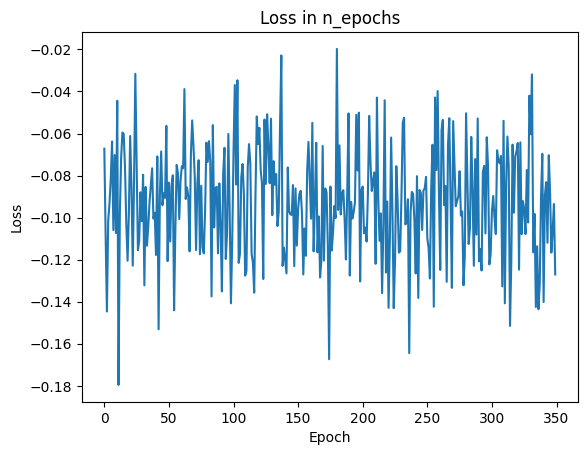
\includegraphics[width=0.7\textwidth]{../figures/4/loss_no_init_fix.png}
    \caption{Função perda sem inicialização adequada - sem aprendizado}
    \label{fig:loss_no_init}
\end{figure}

\begin{figure}[h]
    \centering
    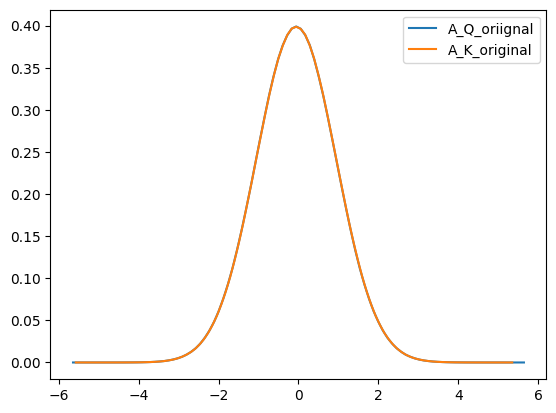
\includegraphics[width=0.7\textwidth]{../figures/4/weight_distributions_no_init_fix.png}
    \caption{Distribuições dos pesos iniciais A\_K e A\_Q}
    \label{fig:weights_no_init}
\end{figure}

\begin{figure}[h]
    \centering
    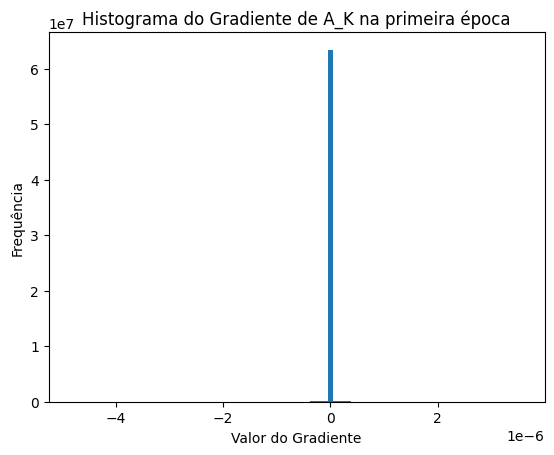
\includegraphics[width=0.45\textwidth]{../figures/4/gradient_histogram_A_K_no_init_fix.png}
    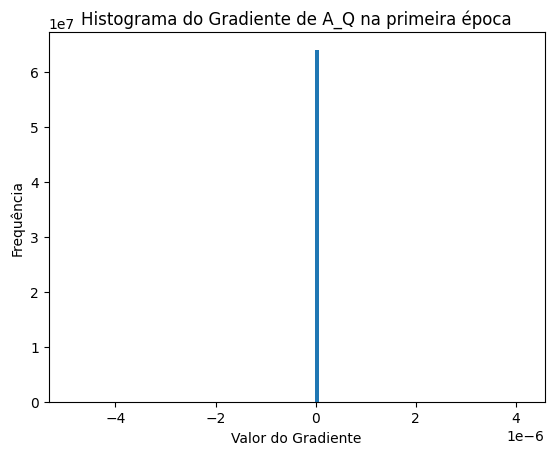
\includegraphics[width=0.45\textwidth]{../figures/4/gradient_histogram_A_Q_no_init_fix.png}
    \caption{Histogramas dos gradientes de A\_K e A\_Q na primeira época (sem inicialização adequada)}
    \label{fig:gradients_no_init}
\end{figure}

\begin{figure}[h]
    \centering
    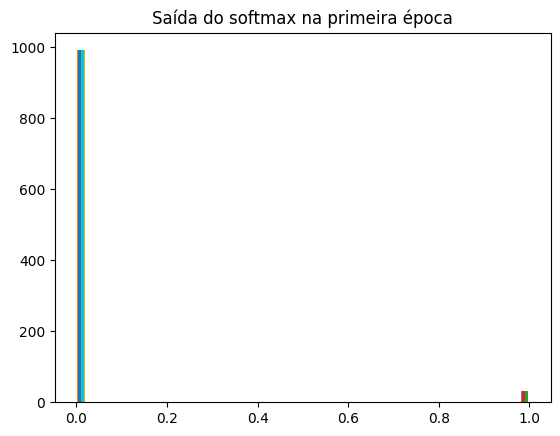
\includegraphics[width=0.7\textwidth]{../figures/4/softmax_output_no_init_fix.png}
    \caption{Saída do softmax na primeira época (sem inicialização adequada)}
    \label{fig:softmax_no_init}
\end{figure}

\vspace{0.5em}
\noindent O c\'{o}digo que demonstra esse problema:

\begin{verbatim}
# Inicialização sem normalização adequada
A_K = torch.randn((D,D)).cuda()  # SEM *init_scale(D)
A_Q = torch.randn((D,D)).cuda()  # SEM *init_scale(D)

# Loop de treinamento
for epoch in range(n_epochs):
    # ... treinamento ...
    att = softmax((K.T@Q)/(D**(1/2)))
    loss = -cos(att,truth).mean()
    loss.backward()
\end{verbatim}
